\newpage
\subsection{Eclipse Plugin}
\subsubsection{Specification and Design}
This section details the implementation to provide a fully integrated development environment in the Eclipse IDE, where developers can explore configuration optimisation and the performance of their applications. From the project deliverables, the following specification is defined:
\begin{itemize}
\item Allow selection of configuration parameters for optimisation - read a list of available parameters for different big data frameworks and dispaly for user selection
\item Depending on the type of selected parameter, its values, ranges and intervals for the experiment to consider can be specified
\item Allow configuration of experiment set-up, connections to remote Jenkins server, remote testbed and monitoring services. Generate formatted experiment configuration file to send.
\item Integrate Eclipse and Jenkins for triggering parameterised builds with configuration files remotely
\item Integrate Eclipse and Jenkins to retrieve and display BO4CO configuration results
\end{itemize}

The main components that form the Eclipse Plugin with the above functionality include:
\begin{itemize}
\item Parser to read available big data framework parameters
\item Eclipse View as the main user interface to display and select parameters
\item Configuration file generator to output experiment configuration
\item Connector to Jenkins to trigger builds and retrieve results
\end{itemize}
The design outlines a user interface with different tabs for parameter selection, services configuration, experiement configuration, application configuration, and experiment execution. The parameter selection tab would show a list of available parameters, filtered by the specific big data framework. Developers can select relevant parameters from the list, and specify ranges or a set of values to test.\\
Parameters may be one of the following types: Integer, Boolean, or Categorical (String). The user interface must be capable of displaying differnt types of parameters with different detailed fields coherently.\\
The required output in the configuration file must follow a strict format to be accepted by the Configuration Optimization tool. The file is in the YAML format, and an example is provided in the \href{https://github.com/dice-project/DICE-Configuration-BO4CO/blob/master/src/conf/expconfig.yaml}{link} \cite{yaml}.

\newpage
\subsubsection{Configuration Parameters}
The Big Data Auto-tuning tool supports four types of configuration parameters: 
\begin{itemize}
\item Integer - the parameter value may be any integer between the \textsc{lower bound} and \textsc{upper bound}, with a user-specified \textsc{step} value that hints to the Configuration Optimising tool the minimum difference between each value to test.
\item Percentage - the parameter value may be any percentage between 0 and 1, with a user-specified \textsc{step} value that hints to the Configuration Optimising tool the minimum difference between each value to test.
\item Boolean - the parameter value may be true or false
\item Categorical - the parameter may take any one of the String values from the  \textsc{options} list
\end{itemize}
In addition to the type specific fields above, all parameters have the following information:
\begin{itemize}
\item name
\item list of applicable big data frameworks
\item default value
\item description
\end{itemize}
The initial implementation had one Parameter class with a \textsc{type} field to distinguish between differnt types of parameters. This was refactorised to the final implementation of a Parameter interface with different implementing classes for each type of parameter. The design choice is discussed in the evaluation section.\\
Parameters available for selection are stored in the \textit{params.xml} file. The XML schema of the file mimics the Java object representation. There are four types of elements for the four types of parameters, with each information field in the parameters stored as a child element in XML. The XML schema can be found in the appendix.\\
The current \textit{params.xml} file contains a selection of configuration parameters from the Apache Hadoop and Apache Storm big data frameworks. These are the two main frameworks supported by the Configuration Optimization tool currently. The configuration parameters included in the file are selected from the officially documented configuration files of the respective frameworks. \cite{hadoopconfig} \cite{stormconfig} The aim is to select \textit{performance related} parameters from the hundreds of parameters. Hence the selection process is based on removing obvious \textit{non-performance related} parameters, such as parameters that:
\begin{itemize}
\item Specifies connections, external inputs and outputs. Eg: file path, service ports
\item Controls security settings, Eg: usernames and passwords
\item Control external functionality. Eg: logging
\end{itemize}
The \textit{params.xml} file can be easily modified to reflect any changes in the parameters of big data frameworks. The file is read every time the Eclipse plugin starts, and any changes to the file will not take effect until the plugin restarts. Because it is data of all available parameters, the plugin never modifies its contents, and treats the file as read-only. The plugin creates a collection of parameter objects internally to temporarily store the parameter information for this session.

\newpage
\subsubsection{User Interface: Parameter Selection}
The parameter selection tab is the most complex and most important tab in the Big Data Auto-tuning tool.\\
\begin{figure}[h]
\centering
\caption{Screen shot of parameter selection tab.}
\label{fig:param}
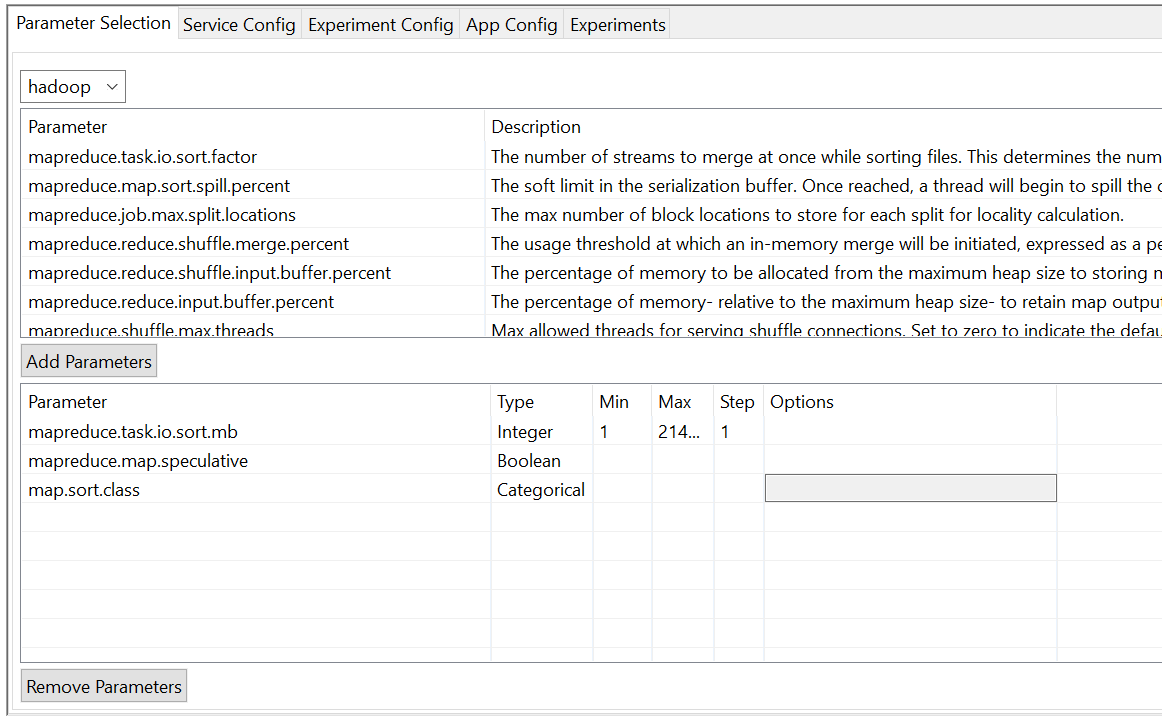
\includegraphics[width=\textwidth]{images/param.png}
\end{figure}
As shown in Figure \ref{fig:param}, two tables form the main part of this tab. The following are the features of the Parameter Selection tab:
\begin{itemize}
\item Upper table displays all parameters available for selection, filtered by the big data framework they are applicable to
\item A second column shows helpful description to explain the purpose of each parameter.
\item The filtering is controlled with the drop-down list on the top left.
\item Parameters available to select can be selected by:
	\begin{itemize}
	\item Double-clicking anywhere on its row
    \item Clicking the row and pressing the ``Add Parameter" button
    \item Multiple parameters can be chosen with common keyboard shortcuts such as ``Ctrl + A'', ``Ctrl + ArrowKey'', and ``Shift + ArrowKey''.
	\end{itemize}
\item Lower table holds the selected parameters
\item Lower table allows the developer to specify values to test each parameter with, instead of showing the description text
\end{itemize}  
The challenge is to allow the developer to specify an arbitrary numerical range for integer and percentage type parameters, and choose from the available options of categorical parameters. There is no need to further restrict the values for Boolean parameters because the choice is binary. The challenge is to display and edit all the different types of details coherently in one table. All text in the table can be edited by double clicking the cell. While the table format is well-suited to taking pure texted based user input, such as the \textsc{min}, \textsc{max}, and \textsc{step}, for numerical inputs, it lacks the built-in ability to display a list of possible options and allow selection of categorical parameter values. A customized drop-down list is created to provide the functionality.\\
\begin{figure}[h]
\centering
\caption{Diagram showing parameter selection tab control and logic.}
\label{fig:paramtab}
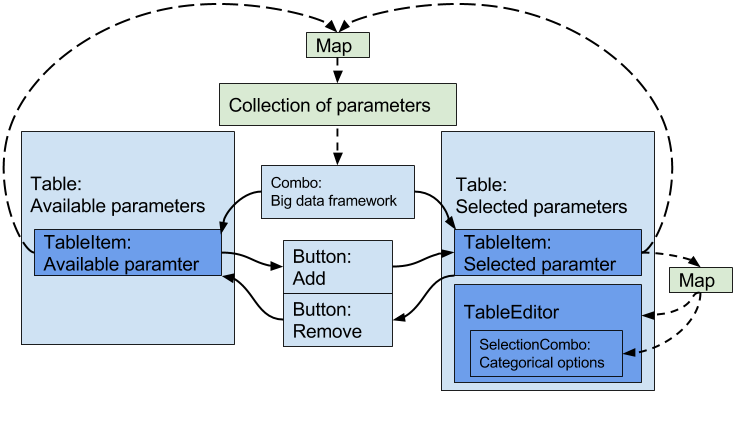
\includegraphics[width=\textwidth]{images/paramtab.png}
\end{figure}
Figure \ref{fig:paramtab} shows how the different components in the parameter selection tab are connected. 
\begin{itemize}
\item Blue components are SWT widgets that appear on the user interface
\item Green components are underlying data collections and objects
\item Deeper shade of blue is used to highlight that multiple instance of the component may exist
\item A SWT widget is the parent of SWT widgets contained inside its box on the diagram
\end{itemize}
When the plugin is launched, a collection of parameter objects is created from reading the \textit{params.xml} file. The SWT Table \cite{swtwidgets} of available parameters is created, along with the drop-down list (SWT Combo \cite{swtwidgets}) that controls which parameters are to be displayed for the selected big data framework. The default selection is for the big data framework first in alphanumeric order. The table is populate with SWT TableItem objects \cite{swtwidgets} that appear as rows on the table. These TableItems are children widgets to the table, and they carry a parameter name and description. Each TableItem is uniquely mapped to the Parameter object that it has been created to display.\\
The SWT Table is a powerful widget, as it contains internally all the logic to detect which items in the table are \textit{selected}. The \textit{selection} may be by mouse click, or by keyboard shortcuts mentioned above.\\
The SWT Table of selected paramters is created to be empty, along with SWT Buttons for ``Add parameter'' and ``Remove parameter''. These buttons will control the movement of parameters across the two tables. Each button has a listener, that listens for a \textsc{MouseDown} event on the button. The listener's \textsc{MouseDown} method is called when the event occurs, so we define the desired action by overriding this method.\\
When the ``Add parameter'' button is pressed:
\begin{enumerate}
\item Query the Table for available parameters for a list of \textit{selected} parameter TableItems
\item Retrieve Parameter objects from mapping of TableItems to Parameter objects
\item Remove \textit{selected} parameter TableItems from the Table for available parameters
\item Create TableItem in the Table for selected parameters for each Parameter object
\item Create a TableEditor to hold the SelectionCombo \cite{mcsc} with corresponding options for each Parameter object of categorical type, and map the TableItem to the SelectionCombo
\end{enumerate}
A double-click listener was added to the Table of available parameters, with the same action of the ``Add parameter'' button, to enable more convenient user selection of parameters.\\
The categorical parameter is the most challenging parameter to display. It requires an arbitrarily long list of options to be shown, but the SWT Table format only supports text in cells of a predefined size. For a coherent user interface, the solution is to use a drop-down list style selection widget that minimizes to a fixed size of a cell. Multiple values from the available options of a categorical parameter has to be selected for experiementation, yet the SWT Combo widget does not allow more than one option to be selected. Therefore a customised widget was created for this purpose. The TableEditor \cite{swtwidgets} allows advanced widgets to be displayed in a cell in a Table, and dynamically manages the display position in relation to a TableItem. However, there is no direct link between the TableItem, TableEditor and the customised widget, which causes problems when one is removed and the other related widgets need to be removed at the same time. Due to this added complexity, the TableItem is mapped to its TableEditor and customised widget.\\
The customised widget is named the MultiCheckSelectionCombo \cite{mcsc}, due to its ability to select multiple values from a drop-down list of check-box styled options. It is similar to a Combo, but built from scratch because SWT conventions dictate that the Combo class cannot be extended. The MultiCheckSelectionCombo is created with support for nearly all of the API of the Combo class, and both sets of Javadocs are available for comparison:
\begin{itemize}
\item Javadoc for MultiCheckSelectionCombo - \href{https://lawhcd.github.io/SWTMultiCheckSelectionCombo/}{link} \cite{javadoc}
\item Javadoc for Combo - \href{http://help.eclipse.org/kepler/index.jsp?topic=\%2Forg.eclipse.platform.doc.isv\%2Freference\%2Fapi\%2Forg\%2Feclipse\%2Fswt\%2Fwidgets\%2FCombo.html}{link} \cite{combo}
\end{itemize}
When the ``Remove parameter'' button is pressed:
\begin{enumerate}
\item Query the Table for selected parameters for a list of \textit{selected} parameter TableItems
\item Retrieve corresponding TableEditor and SelectionCombo objects from mapping and remove them
\item Retrieve Parameter objects from mapping of TableItems to Parameter objects
\item Remove \textit{selected} parameter TableItems from the Table for selected parameters
\item Create TableItem in the Table for available parameters for each Parameter object
\end{enumerate}
The changing of big data framework by selecting a different option on the drop-down list (Combo) is controlled by a \textit{selection} listener. The listener's method is called whenever a new value is \textit{selected}. The action removes all TableItems and related widgets (if any) from both Tables, with similar steps as mentioned above.

\newpage
\subsubsection{User Interface: Services and Configuration}
The Services, Experiment, and Application configuration tabs are similar in that all of the user inputs are simple single text fields. The basic layout structure is a field name (SWT Label \cite{swtwidgets}) followed by a text box (SWT Text \cite{swtwidgets}) for the user to input. The Experiment and Application configuration tabs have no dynamic user interface content that needs to be generated in response to user interaction, and therefore are straight-forward to implement.\\
Although the Services Configuration tab similarly only accepts text input for each field, it requires dynamically generated user interface content, because a user can add an arbitrary number of services to connect to, and each service requires different fields to be specified.\\
\begin{figure}[h]
\centering
\caption{Screen shot of Service Configuration tab.}
\label{fig:services}
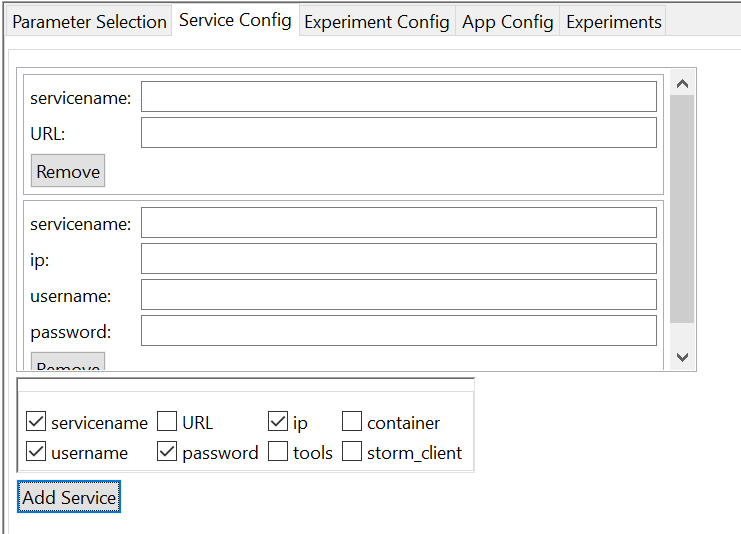
\includegraphics[width=0.8\textwidth]{images/services.png}
\end{figure}
As shown in Figure \ref{fig:services}, the key innovation in the Service Configuration tab is the use of a group of check boxes to customise each new Service. The Service class holds a SWT Text object for each of the 8 possible text fields. Due to the different number of fields that a service can hold, a Service Builder class manages the creation of Services and hides the constructor to prevent errors. When the ``Add Service'' button is pressed, the listener retrieves the selection status of the group of check boxes, and the iteratively builds a service using the Service Builder to create the required fields in the Service. The service is wrapped in a SWT Composite to manage its layout and provide a graphical representation of one coherent unit.

\newpage
\subsubsection{Configuration File Generation}
The experiment configuration file (\textit{expconfig.yaml}) is required input to start the Configuration Optimisation tool (\textit{BO4CO}). The file has four sections corresponding to the details obtained from the user in the Eclipse plugin:
\begin{itemize}
\item Parameters - a selection of big data framework configruation parameters to experiment upon. 
\item Services configuration - details the connections to required services to deploy and monitor the experiment
\item Experiment configuration - settings for experiment time limit, number of iteration and logging options
\item Application configuration - details to enable execution of the big data application for experimentation
\end{itemize}
These information are available in the Eclipse plugin, which holds the set of Parameter objects and a set of user defined Service objects. The experiment and application configurations are not represented as objects, but have their values stored in the SWT Text object fields instead. These are read and collated into arrays of String arguments and passed to the file generator.\\
The file generator outputs these information with correct syntax according to the YAML specification. The overall structure of the file has four mappings for the four sets of details:
\begin{itemize}
\item A YAML Sequence of parameters, where each parameter is a set of simple YAML Scalars for each field.
\item A YAML Sequence of services, where each service is a set of simple YAML Scalars for each field 
\item Two sets of simple YAML Scalars for the other experiemnt and application configurations 
\end{itemize}
Upon testing with the BO4CO Configuration Optimisation tool, it was found that the tool had some flaws and incompleteness in its implementation: 
\begin{itemize}
\item Hard coded reading of services information - The BO4CO code is hard coded to read the sequence of services in a fixed order, as listed here: 
	\begin{enumerate}
	\item Continuous Integration server
    \item DICE Deployment service
    \item DICE Monitoring service
    \item Storm cluster
    \item Kafka
    \item Zookeeper
    \item Hadoop cluster
	\end{enumerate}
In addition the the ordering problem, it also requires that all of the above services be present. That would be a rare case and seems to be a flaw, because a big data application would not typically use Storm and Hadoop frameworks at the same time.\\
The issue was resolved by fixing the ordering of services in the Eclipse plugin, and editing the BO4CO code to remove requirement of multiple big data frameworks.
\item Numerical ranges not supported - The BO4CO configuration file appears to allow the specification of numerical ranges with an upper bound and lower bound. However, the actual code requires that each value for the experiment to be explicitly listed. For example, the range of \textit{``1-5 with step 1''} would have to be listed as the discrete numerical options of \textit{\{1, 2, 3, 4, 5\}}.\\
The issue was resolved by preprocessing numerical range parameters in the Eclipse plugin to generate such list of discrete numerical options.
\end{itemize}





























